%  version 1, 2016-12-05
\documentclass[twocolumn,twoside]{svmultivs_br} %please do not change this line
\usepackage{graphicx}
\usepackage{url}
\usepackage[table]{xcolor}
\usepackage{tabularx}
\usepackage{bm}
\usepackage[multiple]{footmisc}

\title*{Norwegian Mapping Authority Analysis Center Biennial Report}
\subtitle{2019--2020}
\titlerunning{NMA AC 2019--2020 Report}

\author{Ann-Silje Kirkvik}
\authorrunning{Kirkvik} % see comments below
\authoremails{ann-silje.kirkvik@kartverket.no}
\institute{Norwegian Mapping Authority (NMA)}

\component{NMA Analysis Center}

\ContactAuthorName{Ann-Silje Kirkvik}
\ContactAuthorTelephone{+47 32118421}
\ContactAuthorEmail{ann-silje.kirkvik@kartverket.no}
\NumberofInstitutions{1}
\InstitutionPostAddress{1}{Postboks 600 Sentrum, 3507 H\o nefoss}
\InstitutionCountry{1}{Norway}
\InstitutionWebPage{1}{http://www.kartverket.no}

\begin{document}  %please do not change this line
\maketitle       %please do not change this line
\abstract{During 2019 and 2020, the Norwegian Mapping Authority has continued the development of the analysis
software \textbf{Where} that was started in 2015. NMA started to contribute to operational analysis of R1 and R4 
sessions in 2019 and has contributed to the ITRF2020. Work has also been done to scan the antenna dish at NYALES20 
to model the effect of gravitational deformation. The operational analysis is expected to continue and special
attention will be given to the analysis of data from Ny-\AA lesund in the near future.}
\section{General Information}
The Norwegian Mapping Authority (NMA) has been an Associate Analysis Center
within the IVS since 2010. The analysis center is operated by the Geodetic
Institute at NMA with main offices in H\o nefoss, Norway. NMA is a governmental
agency with approximately 800 employees and the IVS activities at NMA are
completely funded by the Norwegian government.

NMA is using the analysis software \textbf{Where}, which is developed at NMA.
\textbf{Where}  and its companion library \textbf{Midgard} is
freely available as open source at GitHub.\footnote{https://kartverket.github.io/where}\footnote{https://kartverket.github.io/midgard}
\textbf{Where} is at the moment
capable of analyzing single sessions of VLBI data, but there is also work underway
to analyze weekly SLR data and some special applications of GNSS.

\subsection{Staff}
The Geodetic Institute at NMA has approximately 50 employees. Some of the responsibilities include maintaining the
national reference frame, geoid and height system. The Geodetic Institute also provides a network-RTK positioning
service and operates the VLBI stations in Ny-\AA lesund \cite{kupiszewski2021}.

The analysis center is organized under a small section named Global Geodesy and in April 2020 Hans Christian Munthe-Kaas
replaced Laila L\o vh\o iden as the section manager. The VLBI analysis group is small and listed in table \ref{tab:staff}.
Development of SLR analysis is led by Ingrid Fausk and development of GNSS applications is led by Michael D\"ahnn.


\begin{table}[htb!]
\caption{VLBI analysis group}
\begin{center}
\begin{tabularx}{\linewidth}{X|X}
\hline
Name  & Role \\
\hline
Ann-Silje Kirkvik & Developer and analyst \\
\AA smund Skj\ae veland & Analyst \\
Leo Olsen & Analyst \\
\hline
\end{tabularx}
\end{center}
\label{tab:staff}
\end{table}

%
\section{Activities during the Past Years}

The years 2019--2020 have certainly been a special period. While 2019 was pretty normal, 2020 was not. In Norway the
whole country went into lockdown the 12th of March due to the global pandemic with the novel coronavirus. Everyone
that was able was sent home and had to work from home. Despite these challenges the operations of the analysis center
and related activities have managed fairly well. 

\subsection{Analysis Center}
%
Towards the end of 2018 analysis results obtained using \textbf{Where} were finally comparable with analysis results
from other established analysis software packages \cite{kirkvik2019}. And in March 2019 the first submissions for
the operational daily SINEX solution started. Shortly afterwards, the version 4 VGOSDB which \textbf{Where} relies upon
to do the analysis became unavailable for approximately two months, but the regular analysis and submissions resumed
in May the same year. Since then, the analyzed R1 and R4 sessions submitted by NMA have been included in the combined
IVS solution. The submitted solutions can be found at the IVS Data Centers with the solution code \texttt{2019a}.
However, on request from the IVS Combination Center (CCIVS) NMA switched to a new solution (\texttt{2020a}) from the
22nd of October 2020 and onwards. The \texttt{2020a} solution is updated with the same models used for the ITRF2020.

The operational R1 and R4 analysis is to some degree automated, but there is still significant room for improvement. 
The observation files are downloaded automatically and the analysis is also started automatically when a new observation
file has been added or an old one has been updated. Files which contain a priori information needed by the analysis is
also downloaded and updated automatically. After the automated analysis is complete some key parameters are investigated.
This is parameters such as variance factor, root mean square, parameter estimates, etc. If any of these parameters are
outside normal values human interaction is needed. If everything is normal the solution is also delivered automatically.
The operational analysis is managed by \AA smund Skj\ae veland.

\subsection{ITRF2020}

The main activity these past two years have been preparation for and analysis of sessions for ITRF2020. \textbf{Where} had
to be updated to support the new models that were required. These models are available from version 1.0.4 of \textbf{Where}
and includes:

\begin{itemize}
  \item New mean pole-tide model
  \item New high frequency EOP model
  \item ICRF3 and galactic aberration
  \item Gravitational deformation of VLBI antennas
\end{itemize}

The IVS contribution to the ITRF2020 includes approximately 6500 S/X sessions and 38 VGOS sessions. This was the first
time all these sessions were analyzed with \textbf{Where} and it was a substantial task to investigate these sessions
to look for clock breaks, outliers and other potential problems. See figure \ref{fig:there} for a screenshot from 
\textbf{There} (the graphical companion program to \textbf{Where}) of a sample
session from the ITRF2020. The final ITRF2020 submission from NMA was delivered at
the beginning of 2021. Development of \textbf{Where} and analysis for ITRF2020 has been done by Ann-Silje Kirkvik.

\begin{figure*}[htb!]
\begin{center}
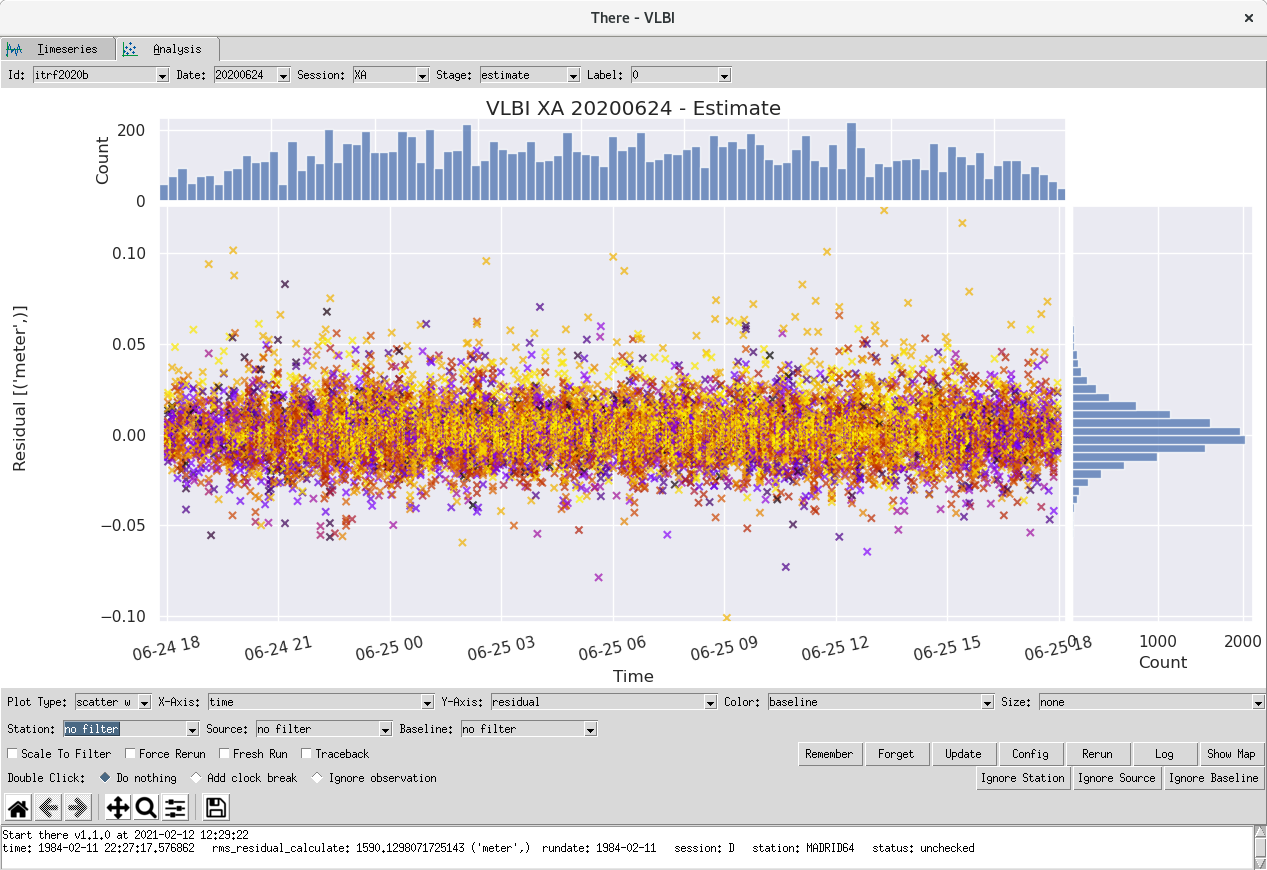
\includegraphics[width=16.0cm]{acnma02.png}
\end{center}
\caption{Postfit residuals (before outlier rejection) for the mixed mode session RD2005 (20JUN24XA). One of thousands
of sessions analyzed for the ITRF2020.}
\label{fig:there}
\end{figure*}

\subsection{Gravitational Deformation Model for NYALES20}
Since gravitational deformation of VLBI antennas were to be included in the analysis for the ITRF2020 and the other
operational products
in the near future, NMA started to investigate the possibilities to do a laser scanning of the antenna at the station
NYALES20. This station has a long
time series going back to 1994 and has participated in many sessions over the years and is therefore an important station
in the network.

NMA did not have the equipment or resources to do this job without aid, and therefore came to an agreement with
the swedish company RISE\footnote{www.ri.se}, which had experience doing a similar job for the station ONSALA60. This
work was lead by Torbj\o rn N\o rbech (retired) from NMA and with the assistanse of the personnel at the station.

The original plan was to do the scanning in May 2020, but travel restrictions all over the world made it impossible to
stick with the original plan. The scanning was postponed to the end of August 2020 and the deformation model became available at the
beginning of November. The model is ready to be applied for the rapid operational products whenever the IVS chooses to
do so. The modelled deformation can be seen in figure \ref{fig:grav_deform}, where the black line $dL$ is the total
change in path length. RISE is working on a publication to document the work that has been done.


\begin{figure*}[htb!]
\begin{center}
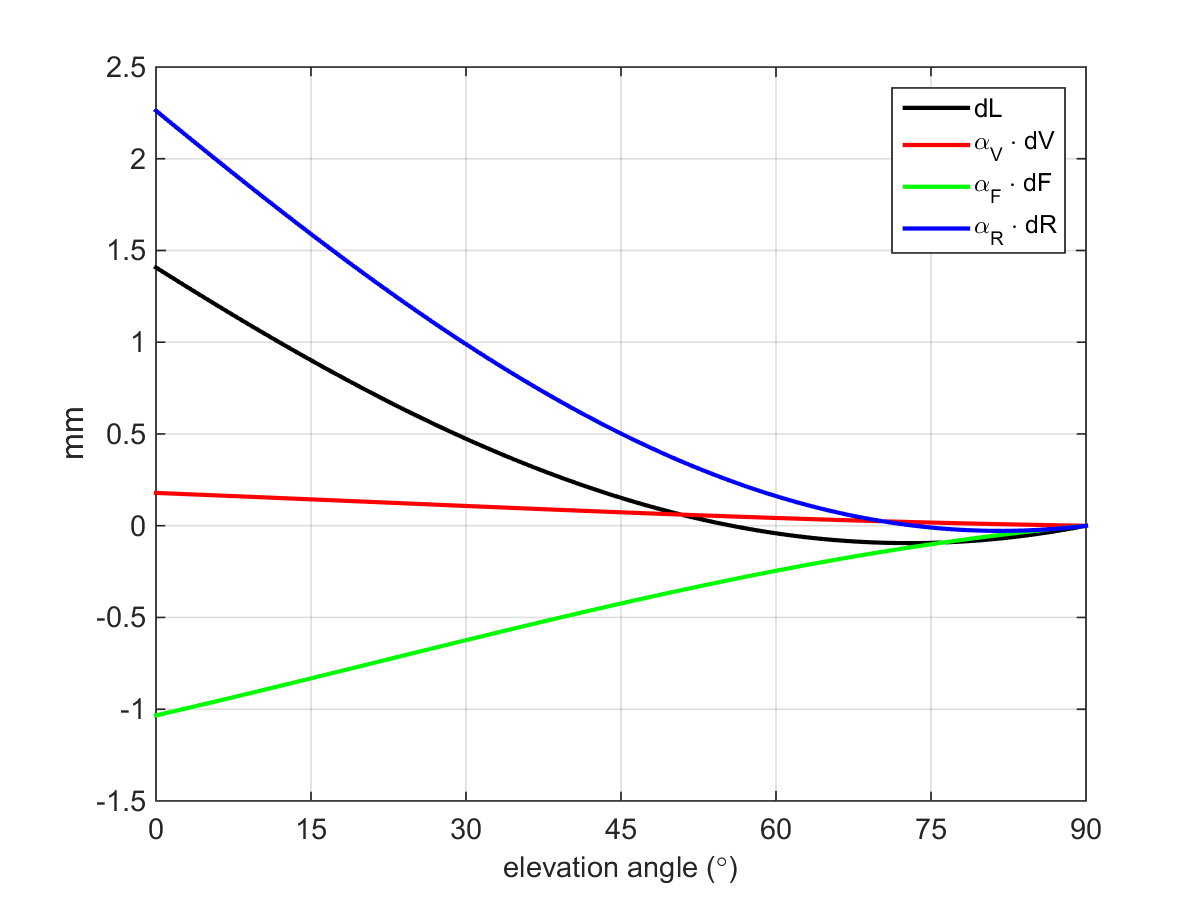
\includegraphics[width=16.0cm]{acnma01.png}
\end{center}
\caption{Gravitational deformation of the NYALES20 antenna. Provided by RISE.}
\label{fig:grav_deform}
\end{figure*}

\subsection{Other news}
The analysis center at IGN (Spain), which is using \textbf{Where}, has also started operational analysis of R1 
and R4 sessions. IGN (Spain) has also recently hired José Carlos Rodriguez, which has experience with SLR analysis from his
previous work and he has been a helpful resourse for Ingrid Fausk with the development of the SLR analysis in 
\textbf{Where}. To facilitate this cooperation the complete SLR code for \textbf{Where} was also released at GitHub
in version 1.1.0. The SLR analysis is not complete and the results should not be used for anything yet, but input
on how to improve the analysis is welcome.    
%
\section{Current Status}
%
The global pandemic is still upon us and as much work as possible is still done from home. The operational analysis is
going smoothly and the ITRF2020 submission is complete.  
%
\section{Future Plans}
%
NMA will continue with the operational analysis of R1 and R4 sessions. With the completion of ITRF2020, the focus
will shift towards investigating the upcoming sessions from Ny-\AA lesund: Both the future VGOS sessions from
NYALE13N and the S/X sessions from NYALES20 and NYALE13S. The latter will be useful to compare the computed baseline
with the measured local tie vector. 

\begin{thebibliography}{99}

\bibitem{kirkvik2019}
A-S.~Kirkvik, ``Norwegian Mapping Authority Analysis Center Biennial Report 2017--2018'',
in \emph{International VLBI Service for Geodesy and Astrometry 2017+2018 Biennial Report},
edited by K. L. Armstrong, K. D. Baver, and D. Behrend,
NASA/TP-2020-219041, 2020.
\bibitem{kupiszewski2021}
P.~Kupiszewski, ``Ny-\AA lesund Geodetic Observatory'',
in \emph{International VLBI Service for Geodesy and Astrometry 2019+2020 Biennial Report},
edited by K. L. Armstrong, K. D. Baver, and D. Behrend,
this volume.
\end{thebibliography}
%
\end{document}
